\chapter{Podstawy teoretyczne}
\label{cha:teoria}

W rozdziale tym przedstawione zostaną zagadnienia ściśle związane z tematem tej pracy, których znajomość niezbędna jest do zrozumienia kolejnych rozdziałów. 



%---------------------------------------------------------------------------

\section{Wzrost zagrożeń w globalnej sieci Internet}
\label{sec:penTest}

Obecnie sieci IP są w znaczym stopniu zabezpieczone w sposób niewystarczający, co za tym idzie, hakerzy są w stanie wykorzystać istniejące luki w ich infrastrukturze do uzyskania nieautoryzowanego dostępu do wrażliwych danych przedsiębiorstw w celu zakłócenia prawidłowego ich działania %działania serwisów sieciowych. 


Zgodnie z danymi przedstawionymi w raporcie amerykańskiego Federalnego Biura Śledczego, departament  Internet Crime Complaint Center (IC3), \cite{FBI2015} z roku na rok wzrasta ilość strat poniesionych w wyniku cyber-przestępstw ustalając się w roku 2015 na poziomie 1,070.71 milionów dolarów amerykańskich co w porównaniu z rokiem 2001 (17.8 milionów USD) wynosi wzrost o ponad 600 procent. W związku z tak gwałtownym wzrostem strat poniesionych przez przedsiębiorstwa narasta potrzeba zabezpieczenia wrażliwych na ataki infrastuktur informatyczych. 


Instnieją różne sposoby sprawdzenia poziomu bezpieczeństwa instniejącej sieci. Dla przykładu "network vulnerability assessments" badają każdy komponent sieci próbując "determine" szeroką gamę podatności i luk. "Automated vulnerability
scanners" mogą być użyte do rutynowej kontroli sieci i ostatecznie testy penetracyjne testują, czy zabezpieczenia danej sieci mogą być złamane w danym przedziale czasowym.




%---------------------------------------------------------------------------

\section{Czym są testy penetracyjne}
\label{sec:penTest}

Zgodnie z definicją \cite{He2006}, testy penetracyjne sieci są sposobem dla przedsiębiorstw i innych organizacji do odnalezienia luk w zabezpieczenia na tyle wcześnie, aby zapobiec wykorzystaniu ich przez hakerów do włamania się i kradzieży istotnych dla firmy danych i informacji. Informacje te mogą przejawiać się w wielu różnych formach, takich jak własność intelektualna, kod źródłowy lub jego dokumentacja czy też nazwy użytkowników i ich hasła, niezależnie jednak od formy, są to dane na których organizacja ta w znaczym stopniu się opiera i powinny być one chronione (?)\cite{}. 

% Organizations will spend a lot of time and resources trying to protect themselves from these attacks. They will implement firewalls to keep attackers out and intrusion detection systems to hopefully catch when someone gets through the firewall. They will also implement procedures within the organization to protect themselves from insider attacks, which are also common. This may include the requirement of strong passwords or perhaps multi-factor authentication, which may require the user to have something on them or even use something like a fingerprint in addition to using a username and password. The thing that organizations are trying to protect against is vulnerability. A vulnerability is a weakness in a system. System , though, is a very vague term. By using the word system , in this case, we are not only talking about the operating system and applications that make your computer useful but also, in a larger context, all of the computers and network devices within the entire enterprise network. The organization will try to locate its weaknesses, or vulnerabilities, and either remove or reduce them. The process of trying to remove or reduce a vulnerability is called remediation . When you are trying to reduce the impact of a vulnerability being taken advantage of, you are mitigating the impact. So, in the process of managing vulnerabilities, you will hear the terms mitigation and remediation \cite{}.

% When you take advantage of a vulnerability, you are exploiting it. You will see references to exploits as we continue, which are specific techniques or even pieces of software that are designed to exploit a particular vulnerability. The point of an exploit may be to obtain system-level access, meaning the attacker can see and even control files, users, and services

% The last thing to go over, while we are talking about information security and vulnerability management, is the idea of probability and impact. When assessing a vulnerability, a security professional will generally take into account two factors. The first is the probability. This is often given a qualitative valuation like low, medium, or high. What it refers to is the likelihood of a particular vulnerability being exploited. If there is proof-of-concept code available or if there is flat out an exploit widely available (“in the wild”), the likelihood may be very high. If you have additional mitigations in place, like you have to be on the local network and not remote in order to take advantage of the vulnerability, you may decide the probability is lower. Making this valuation and categorization will often take a combination of knowledge and experience. The other factor that is important to know about is the impact. This is what happens if the exploit is triggered. If the exploit causes the application to crash but it comes right back up, this is probably a low-impact exploit. If, on the other hand, it causes a remote attacker to get unauthorized administrative access to your system, the impact is high. If it causes the destruction of critical or sensitive information for the business, you may also say it’s high impact. While this may be easier to gauge than probability, it still takes a fair amount of knowledge and experience to be able to do it accurately.

% One last thing to note. We have been talking about information security, and that’s a phrase you will hear about a lot. The objective is to protect the information assets of an organization. However, an attacker may not care about your information assets. They may care more about your computing assets. In other words, they may simply be looking to collect a system they can add to their network of systems that will perform tasks for them. This is a very lucrative business, so don’t assume that just because you are a small organization you aren’t a target. You are. Especially if you are easy for the picking. Your systems and their computing power are just as good as those from large, high-profile companies — more so if they are easy to break into



Ważnym pojęciem w tym temacie są tak zwani "etyczni hakerzy" - osoby zatrudniane do włamania się do sieci a następnie przeprowadzenia licznych ataków przy użyciu technik, które mogą wykorzystać przestępcy internetowi (?).


Bazowo rozróżniamy dwa typy testów penetracyjnych \cite{Klev04}:
\begin{enumerate}
\item testy zapowiedziane (announced testing) - próba przechwycenia wyszczególnionych wcześniej plików będących "flagami" lub też próba skompromitowania systemów w sieci klienta korzystająć z pełnej kooperacji z zespołem technicznym, dokumentacji projektowej lub kodu źródłowego,

\item testy niezapowiedziane (unannounced testing) - różni się od testów zapowiedzianych tym, że jedynie "upper levels of management" jest poinformowany o tym fakcie. Tego typu testy sprawdzają procedury bezpieczeństwa, instniejącą infrastrukturę bezpieczeństwa a także "reaktywność" pracowników.
\end{enumerate}

Ponadto możemy rozrózniać \cite{Geer02},\cite{Messier2016}:
\begin{enumerate}
\item test penetracyjny z minimalną wiedzą (black box) w którym konsultanci bezpieczeństwa nie mają wcześniejszej wiedzy na temat sieci którą mają penetrować, poza informacją, która sieć jest ich celem. Wymaga to poświęcenia sporej ilości czasu w fazie przygotowawczej, jest to jednak etap wartościowy dla klienta, ponieważ dostarcza informacji na temat danych, które są dostępne na jego temat dla outside world %This means that the team has to spend a considerable amount of time trying to discover such information.

\item test penetracyjny z pełną wiedzą (crystal box, white box) gdzie zespół posiada kluczowe informacje na temat sieci będącej celem, jej konfiguracji a także dane na temat oprogramowania i sprzętu będącego w użyciu firmy. W cały proces zaangażowany jest także presonel firmy zapewniający szczegółowe informacje na temat systemu i kontolujący jego dziłanie w czasie trwania testów aby nie sprawiały one problemów dla zwykłych użytkowników. %The first is because the attacker is going to keep poking and prodding until something eventually gives. Second, some attacks happen from the inside. These people will know about some of these settings and be able to make use of them. ... You may have systems that appear to be very hard on the outside, but once the system is popped..

\item testy penetracyjne z częściową wiedzą (grey box) znajdujący się pomiędzy wcześniejszymi dwoma. W tym typie testu, zespół posidada podstawowe informacje na temat testowanej sieci takie jak adres IP czy nazwa hosta. Dzięki temu testerzy nie muszą poświecać tak wiele czasu na uzyskiwanie podstawowych informacji i mogę dokładniej zbadać inne istotne moduły systemu.
\end{enumerate}

%Determining how you plan to approach should ideally be based on an intersection of the amount of time you have and what the client is really looking to accomplish.

% Typically, testing is performed in a production environment . This provides the best idea of how good the defenses are in the live systems. There is a risk to this, however. Some companies may prefer some of the testing to be done in a protected lab environment to avoid any impact to the live systems.

%In this section the general process of a penetration test is illustrated with the help of figure 1 [2]. Professional testers have to compromise a network in a given period of time, finding as many weaknesses as possible, so a well-defined methodology to sys- tematically check for known vulnerabilities and pursue potential security holes is critical. The importance of a common methodology is further stressed in [5]. Figure 1 shows the four-step process in a typical penetration test.

% source = Lam, F., Beekey, M., and Cayo, K.: Can you hack it? Security Management, vol. 47 no. 2,pp. 83-88, Feb 2003.

\begin{figure}
  \caption{Schemat procesu testu penetracyjnego (?)}
    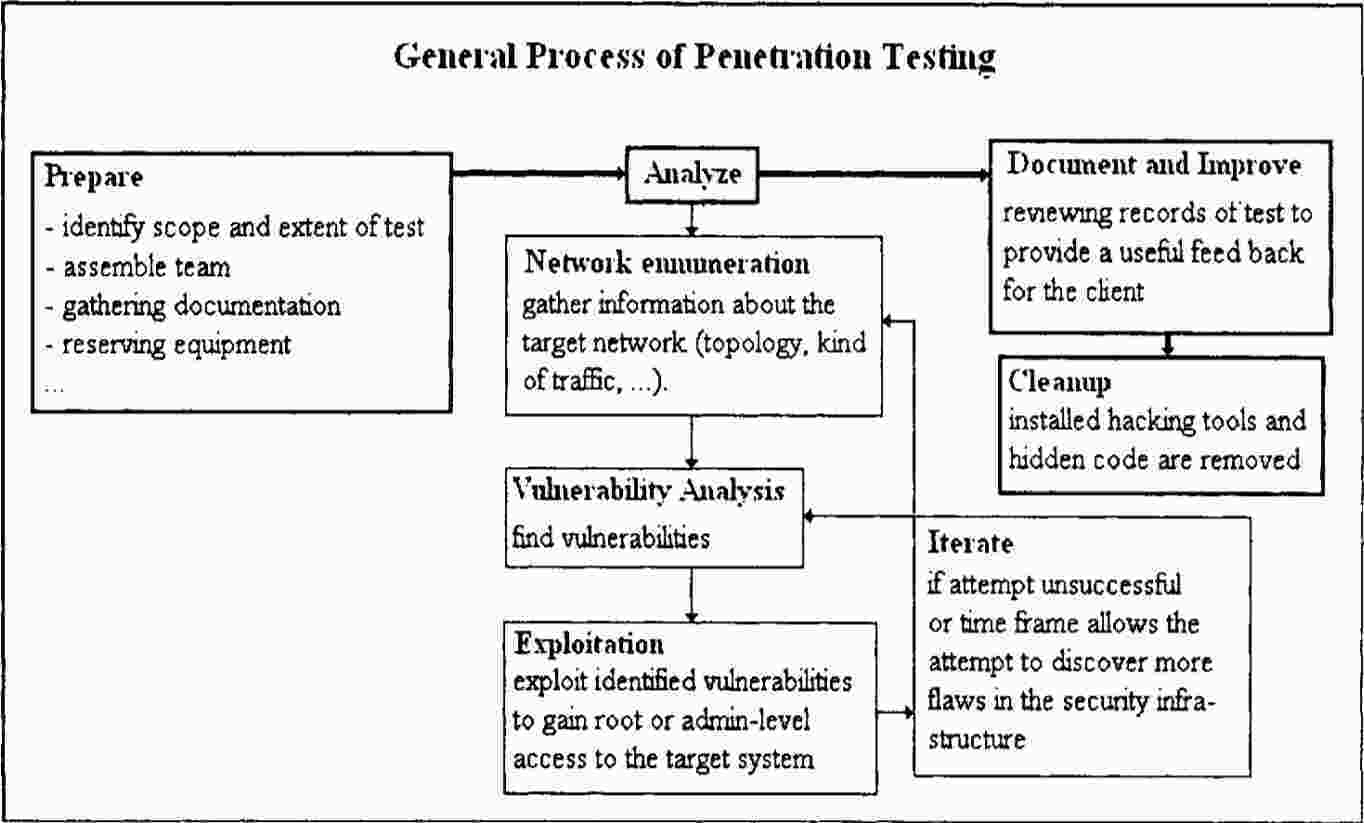
\includegraphics{others/pentest_process}
\end{figure}


istotne jest aby po skończoncyh testach penetracyjnych dostarczyć do klienta dokładny raport z wynikami, jakie po testach tych udało się osiągnąć

%- - - - - 

%Test penetracyjny z minimalną wiedzą (black box) – w największym stopniu stara się odzwierciedlić rzeczywistą wiedzę potencjalnego włamywacza, w związku z czym zespół testujący otrzymuje np. wyłącznie adres serwisu i nic ponadto. Wadą tej metody jest możliwość poświęcenia przez zespół nieproporcjonalnie dużych ilości czasu na działania bezproduktywne, np. próbę złamania hasła na wejściu do serwisu w sytuacji, gdy autentyczny włamywacz mógłby tę wiedzę zdobyć innymi metodami (np. za pomocą phishingu lub metod wiążących się ze złamaniem prawa)

%Announced testing is an attempt to access and retrieve pre-identified flag file(s) or to compromise systems on the client network with the full o-operation and knowledge of the IT staff. Such a test examines the existing security infrastructure and individual systems for possible vulnerabilities.

%Test penetracyjny z pełną wiedzą (crystal box) – zespół testujący ma pełny dostęp do dokumentacji projektowej, kodu źródłowego, konfiguracji urządzeń sieciowych itd. W przypadku opierania się wyłącznie na tej wiedzy można mówić o „przeglądzie kodu” lub „przeglądzie konfiguracji”. Wadą takiego podejścia jest możliwość pominięcia rozbieżności pomiędzy stanem udokumentowanym a stanem faktycznym.


%---------------------------------------------------------------------------

\subsection{Rozwój testów penetracyjnych}

<charakter> testów penetracyjnych w znacznej mierze zależy od ewolucji narzędzi służących do hackingu a używanych przez cyber-przestępców. Bazowa struktura pentestingu jest jednak stała i składa się z czterech faz (Przygotowania, Analiza, Dokumentacja i Cleanup). Jednakże używane techniki oraz nasick <balans rozkład> mogą ulegać zmianie zależnie od pojawiania się nowych wątków w tematyce bezbieczeństwa sieciowego pojawiających się se wględu na rozwój coraz bardziejzłożonych narzędzi służącyhc ddo hackingu, potrzeb redukowania kosztów jak rówież wprowadzania nowych typów sieci



%---------------------------------------------------------------------------

\section{przykład scenariusza pentestingu}
\label{sec:zawartoscPracy}

todo

%Wsasasaas rodziale \ref{cha:wprowadzenie} przedstawiono podstawowe informacje dotyczące struktury dokumentów w \LaTeX u. Alvis~\cite{Alvis2011} jest językiem


\section{Na czym polega scanning?}

Scanning – this is a different level of reconnaissance. Before
you start determining your attack strategy, you need to know
what your targets are. This will provide you with a lot of
information about systems and ports as well as, potentially,
any firewalls that may be in place. This is also where you may
need to exercise caution, depending on what level of testing
you are performing. This can be a very noisy step, since you
are starting to engage directly with the target here. It may be
useful for the client to see if they can detect the scanning as
part of shoring up their defensive stance.

